<<<<<<< HEAD
\section{Background and Motivation}
\subsection{Workloads}

\subsection{Motivation}
Consider a scenario for running the image recognition application on mobile platform.
Here we running the inference tasks on
two typical models: $VGG\_16$ and $Resnet50$ as background 
support on the NVIDIA Jetson TX2 embedded deep learning platform.
Afther that, we compress both $VGG\_16$ and $Resnet50$ by using pruning 
and quantization respectively, and then deploy them on the same platform
and running the same inference tasks.
In this work, we consider the
model size, inference time and accuracy before and after the compression.

\cparagraph{Testing set.}
We use 50000 pictures from Imagenet as test set
which includes 1000 categories,
and feed them into the $VGG\_16$ and $Resnet50$ respectively. 
We repeat this procedure 10 times for each picture
and record the inference time and the predicted result.
Finally, we calculate the average value of inference time and accuracy
for each model.

\cparagraph{Motivation Results.}
Figure\ref{fig:motivation} compares the model size, inference time and accuracy of the default
$VGG\_16$ and $Resnet50$ and the compressed ones via different techniques.
For model size, the quantization perform the best which gives 75\% and 74.8\%
reduction for $VGG\_16$ and $Resnet50$ respectively when compared with the default model. 
The pruning only delivers an average of xxx\% reduction for both of them.
For inference time, we can see the purning achieves an averaged speedup of 1.28x,
on the contrary, the quantization causes significant slowdown with 1.45x than the default model,
the details will be disscused in section \FIXME{};
As for accuracy,  the overall accuracy of pruning drops only 5\%, the quantization drops 3\%.
So we can maintain the default value when using the above mentioned two compression techiniques.
=======

\section{Motivation}
Compressing a deep learning model into a smaller size typically leads to a smaller model footprint, but it does not always lead to faster
inference time and lower energy consumption. As a motivation example, considering applying \FIXME{four} commonly used model compression
techniques to \FIXME{xx} influential deep learning models -- including \FIXME{xx} \CNNs and \FIXME{RNNs}. Our evaluation platform is a
NVIDIA Jetson TX2 embedded deep learning platform with Tensorflow Mobile \FIXME{v.xx} (see Section~\ref{sec:platform}).

Figure~\ref{} summarizes the change of the storage size, memory footprint, inference time, and energy consumption after applying each model
compression technique.

\ref{fig:motivation}

>>>>>>> 807861a1dc9987c65b37af9de20b0b63329e0e33
\begin{figure}[!t]
\centering
\subfloat[][Model size]{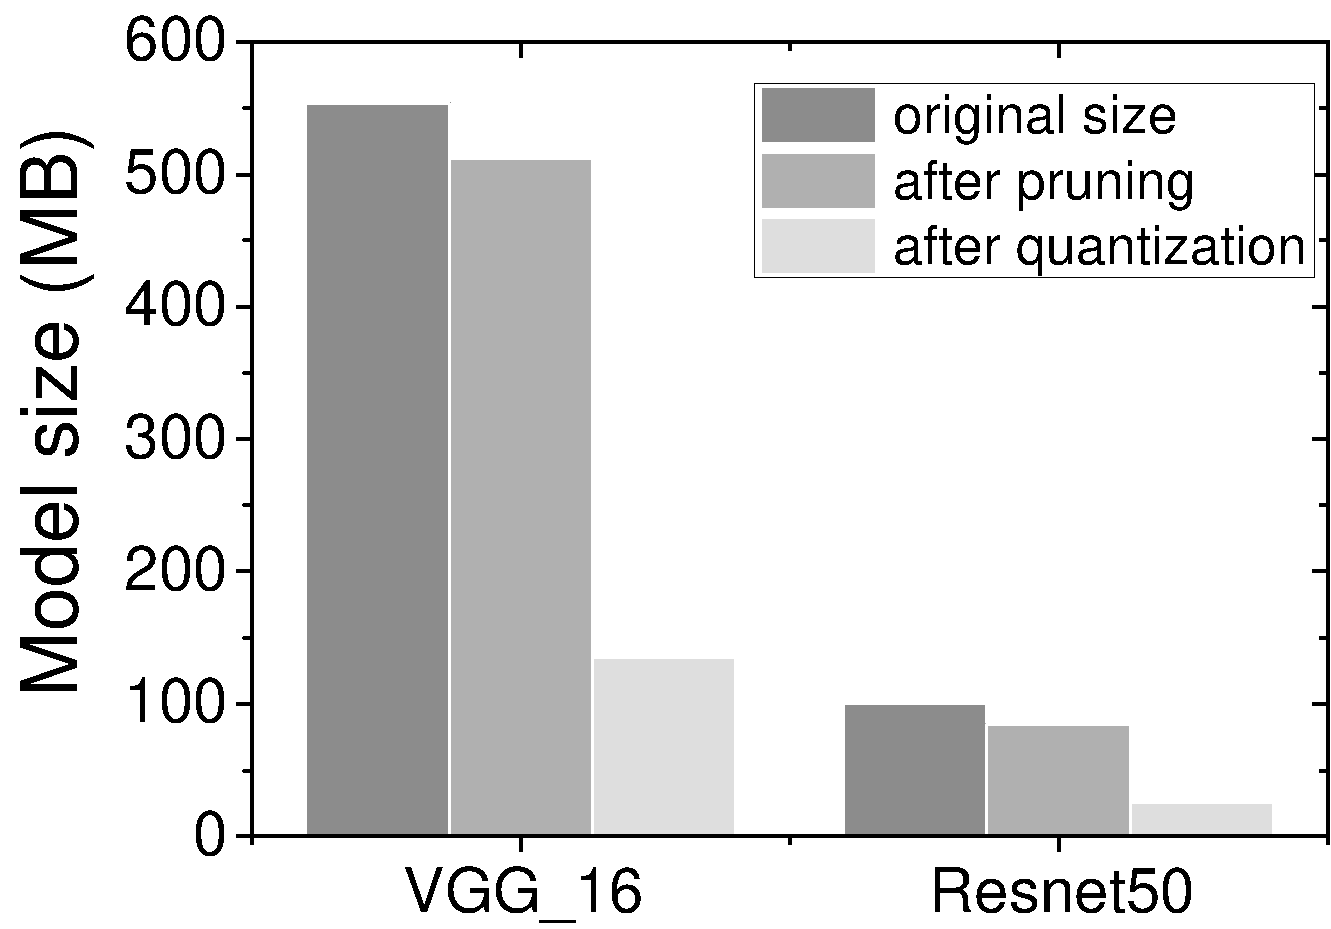
\includegraphics[width=0.33\textwidth]{figure/motivation_size.pdf}}
\hfill
\subfloat[][Inference time]{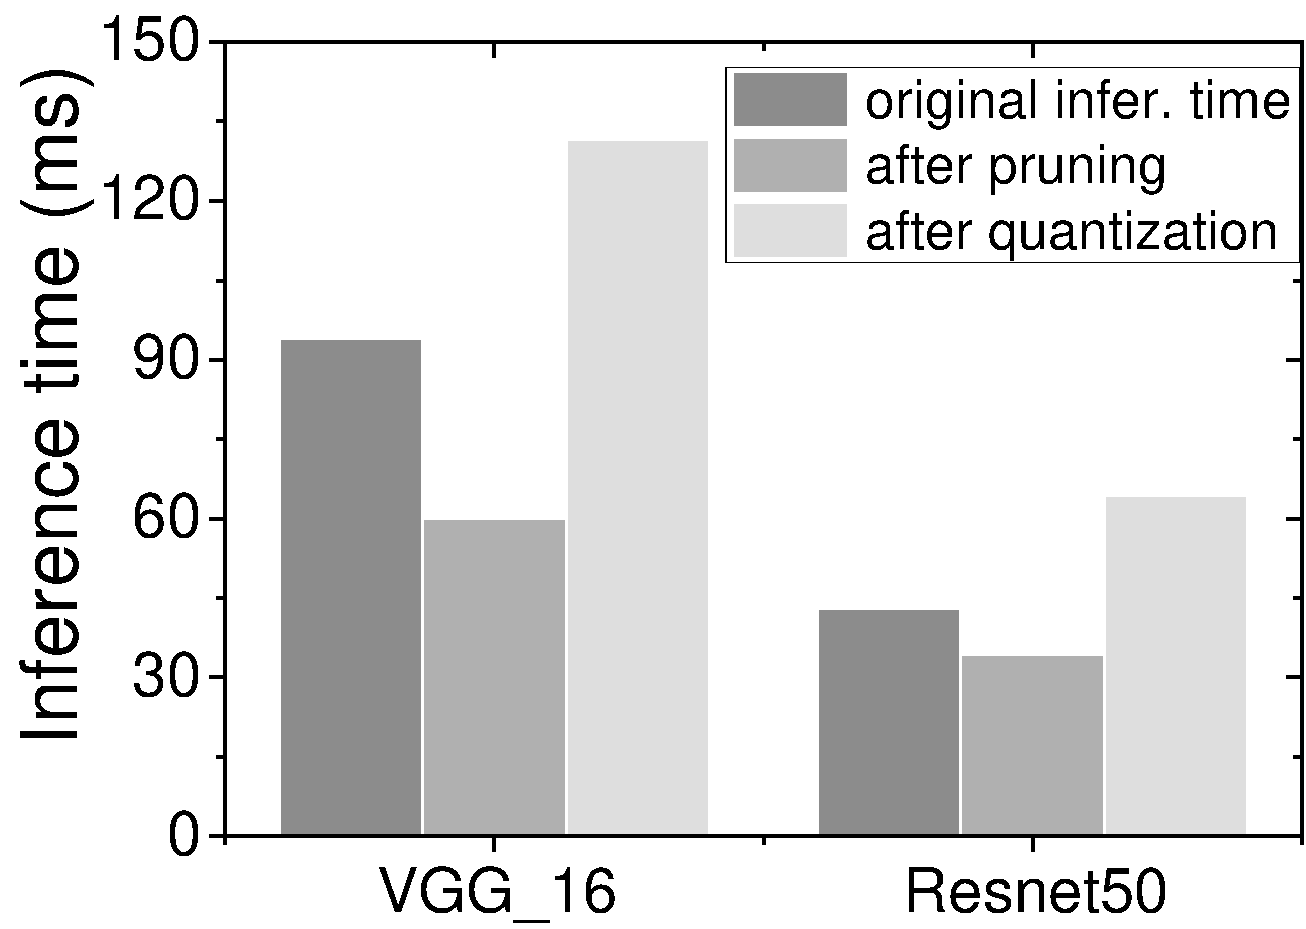
\includegraphics[width=0.33\textwidth]{figure/motivation_time.pdf}}
\hfill
<<<<<<< HEAD
\subfloat[][Accuracy]{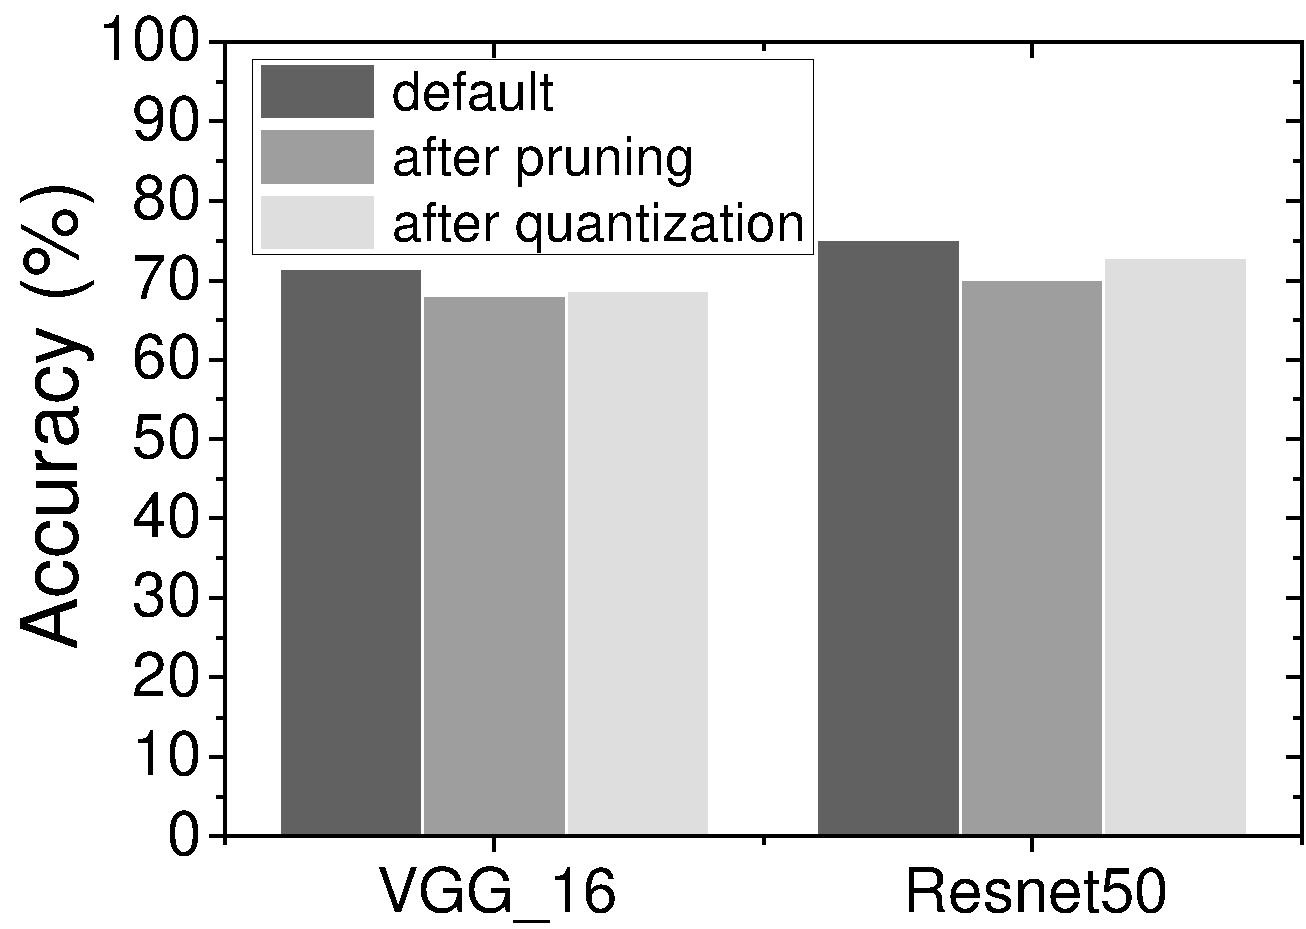
\includegraphics[width=0.33\textwidth]{figure/motivation_accuracy.pdf}}
\caption{The achieved model size (a) inference time (b) and accuracy (c) before and after the compression by quantization and pruning.
There is significant room for improvement.} 
\label{fig:motivation}
\end{figure}

\cparagraph{Lesson Learned.}
This example shows that the current models are ill-suited for mobile platform,
expecially the high price for memory usage and energy.
The compression techniques have different effects depends on the model 
structure.
The quantization outperforms prunning in compression radio by
reducing the number of bits of each float value, while the inference time increasd.
The pruning fouces on the removing the redundent parameters which have little effect 
on the default structure.
There is a need for a better compressed
model that can adapt to the mobile platform. In the remainder of this
paper, we describe such an approach based on the above mentioned techiques.



=======
\subfloat[][Inference time]{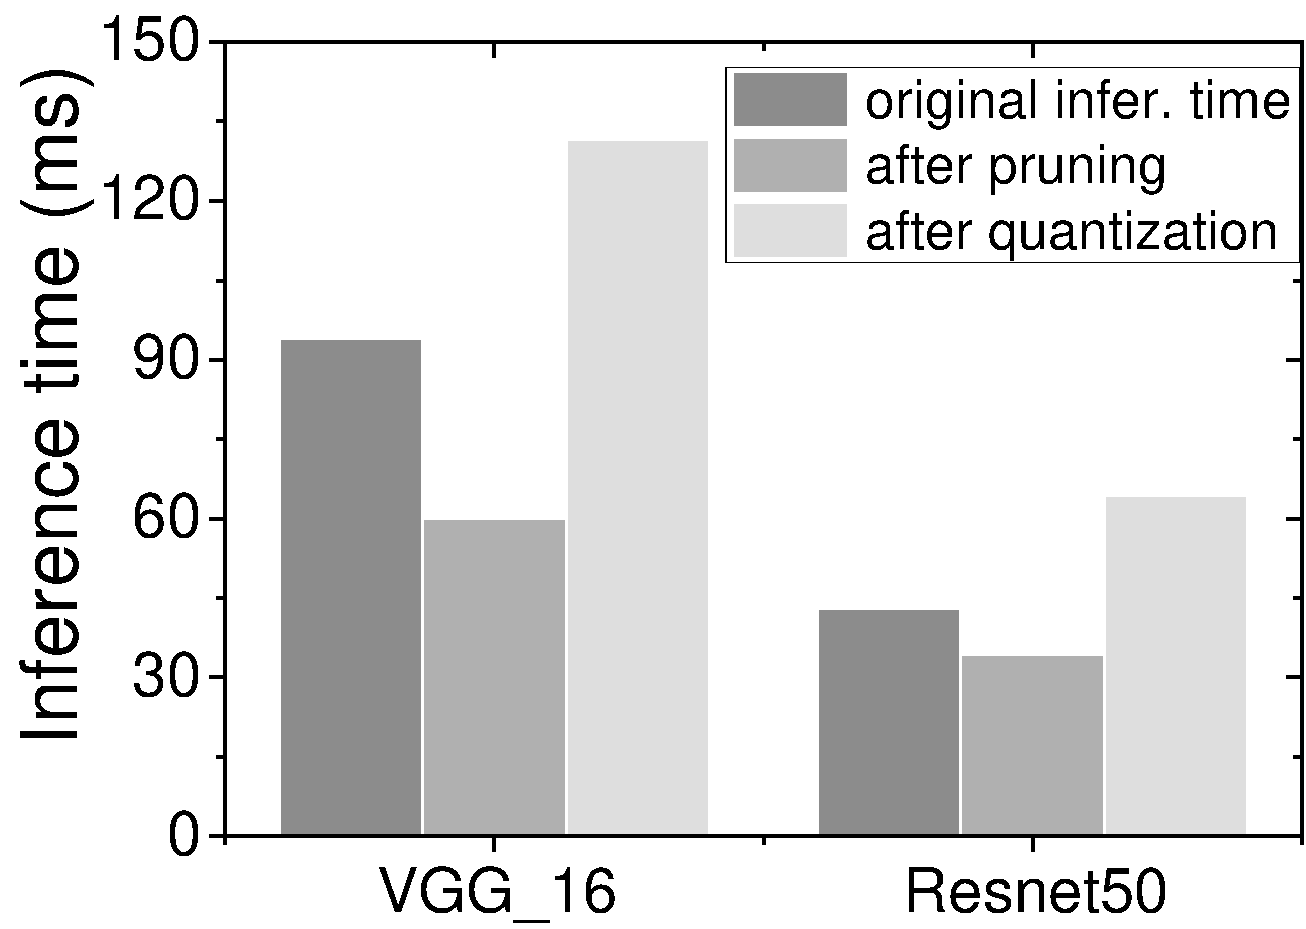
\includegraphics[width=0.4\textwidth]{figure/motivation_time.pdf}}
\caption{The achieved model size (a) and inference time (b) before and after the compression by quantization and pruning.
There is significant room for improvement.}
\label{fig:motivation}
\end{figure}
>>>>>>> origin/master
>>>>>>> 807861a1dc9987c65b37af9de20b0b63329e0e33
